% Created by tikzDevice version 0.6.2-92-0ad2792 on 2013-02-15 17:08:39
% !TEX encoding = UTF-8 Unicode
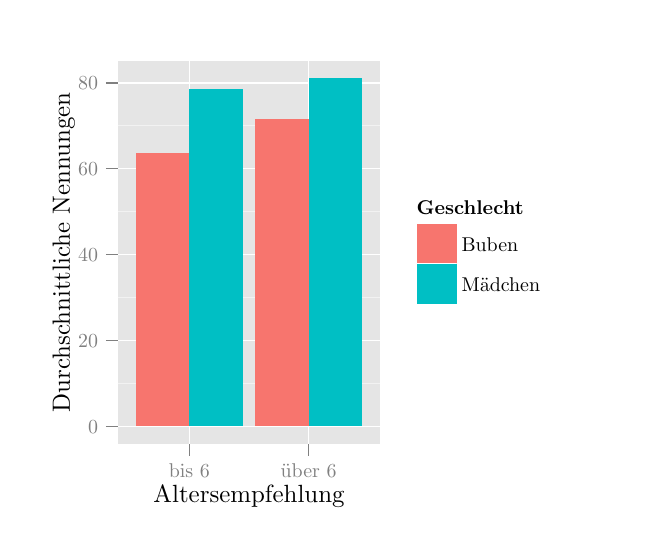
\begin{tikzpicture}[x=1pt,y=1pt]
\definecolor[named]{fillColor}{rgb}{1.00,1.00,1.00}
\path[use as bounding box,fill=fillColor,fill opacity=0.00] (0,0) rectangle (216.81,180.67);
\begin{scope}
\path[clip] (  0.00,  0.00) rectangle (216.81,180.67);
\definecolor[named]{drawColor}{rgb}{1.00,1.00,1.00}
\definecolor[named]{fillColor}{rgb}{1.00,1.00,1.00}

\path[draw=drawColor,line width= 0.6pt,line join=round,line cap=round,fill=fillColor] (  0.00,  0.00) rectangle (216.81,180.67);
\end{scope}
\begin{scope}
\path[clip] ( 32.55, 30.32) rectangle (127.38,168.63);
\definecolor[named]{fillColor}{rgb}{0.90,0.90,0.90}

\path[fill=fillColor] ( 32.55, 30.32) rectangle (127.38,168.63);
\definecolor[named]{drawColor}{rgb}{0.95,0.95,0.95}

\path[draw=drawColor,line width= 0.3pt,line join=round] ( 32.55, 52.13) --
	(127.38, 52.13);

\path[draw=drawColor,line width= 0.3pt,line join=round] ( 32.55, 83.17) --
	(127.38, 83.17);

\path[draw=drawColor,line width= 0.3pt,line join=round] ( 32.55,114.22) --
	(127.38,114.22);

\path[draw=drawColor,line width= 0.3pt,line join=round] ( 32.55,145.27) --
	(127.38,145.27);
\definecolor[named]{drawColor}{rgb}{1.00,1.00,1.00}

\path[draw=drawColor,line width= 0.6pt,line join=round] ( 32.55, 36.60) --
	(127.38, 36.60);

\path[draw=drawColor,line width= 0.6pt,line join=round] ( 32.55, 67.65) --
	(127.38, 67.65);

\path[draw=drawColor,line width= 0.6pt,line join=round] ( 32.55, 98.70) --
	(127.38, 98.70);

\path[draw=drawColor,line width= 0.6pt,line join=round] ( 32.55,129.74) --
	(127.38,129.74);

\path[draw=drawColor,line width= 0.6pt,line join=round] ( 32.55,160.79) --
	(127.38,160.79);

\path[draw=drawColor,line width= 0.6pt,line join=round] ( 58.42, 30.32) --
	( 58.42,168.63);

\path[draw=drawColor,line width= 0.6pt,line join=round] (101.52, 30.32) --
	(101.52,168.63);
\definecolor[named]{fillColor}{rgb}{0.97,0.46,0.43}

\path[fill=fillColor] ( 39.02, 36.60) rectangle ( 58.42,135.52);
\definecolor[named]{fillColor}{rgb}{0.00,0.75,0.77}

\path[fill=fillColor] ( 58.42, 36.60) rectangle ( 77.81,158.38);
\definecolor[named]{fillColor}{rgb}{0.97,0.46,0.43}

\path[fill=fillColor] ( 82.12, 36.60) rectangle (101.52,147.60);
\definecolor[named]{fillColor}{rgb}{0.00,0.75,0.77}

\path[fill=fillColor] (101.52, 36.60) rectangle (120.92,162.34);
\end{scope}
\begin{scope}
\path[clip] (  0.00,  0.00) rectangle (216.81,180.67);
\definecolor[named]{drawColor}{rgb}{0.50,0.50,0.50}

\node[text=drawColor,anchor=base east,inner sep=0pt, outer sep=0pt, scale=  0.72] at ( 25.44, 34.12) {0};

\node[text=drawColor,anchor=base east,inner sep=0pt, outer sep=0pt, scale=  0.72] at ( 25.44, 65.17) {20};

\node[text=drawColor,anchor=base east,inner sep=0pt, outer sep=0pt, scale=  0.72] at ( 25.44, 96.22) {40};

\node[text=drawColor,anchor=base east,inner sep=0pt, outer sep=0pt, scale=  0.72] at ( 25.44,127.26) {60};

\node[text=drawColor,anchor=base east,inner sep=0pt, outer sep=0pt, scale=  0.72] at ( 25.44,158.31) {80};
\end{scope}
\begin{scope}
\path[clip] (  0.00,  0.00) rectangle (216.81,180.67);
\definecolor[named]{drawColor}{rgb}{0.50,0.50,0.50}

\path[draw=drawColor,line width= 0.6pt,line join=round] ( 28.29, 36.60) --
	( 32.55, 36.60);

\path[draw=drawColor,line width= 0.6pt,line join=round] ( 28.29, 67.65) --
	( 32.55, 67.65);

\path[draw=drawColor,line width= 0.6pt,line join=round] ( 28.29, 98.70) --
	( 32.55, 98.70);

\path[draw=drawColor,line width= 0.6pt,line join=round] ( 28.29,129.74) --
	( 32.55,129.74);

\path[draw=drawColor,line width= 0.6pt,line join=round] ( 28.29,160.79) --
	( 32.55,160.79);
\end{scope}
\begin{scope}
\path[clip] (  0.00,  0.00) rectangle (216.81,180.67);
\definecolor[named]{drawColor}{rgb}{0.50,0.50,0.50}

\path[draw=drawColor,line width= 0.6pt,line join=round] ( 58.42, 26.05) --
	( 58.42, 30.32);

\path[draw=drawColor,line width= 0.6pt,line join=round] (101.52, 26.05) --
	(101.52, 30.32);
\end{scope}
\begin{scope}
\path[clip] (  0.00,  0.00) rectangle (216.81,180.67);
\definecolor[named]{drawColor}{rgb}{0.50,0.50,0.50}

\node[text=drawColor,anchor=base,inner sep=0pt, outer sep=0pt, scale=  0.72] at ( 58.42, 18.24) {bis 6};

\node[text=drawColor,anchor=base,inner sep=0pt, outer sep=0pt, scale=  0.72] at (101.52, 18.24) {über 6};
\end{scope}
\begin{scope}
\path[clip] (  0.00,  0.00) rectangle (216.81,180.67);
\definecolor[named]{drawColor}{rgb}{0.00,0.00,0.00}

\node[text=drawColor,anchor=base,inner sep=0pt, outer sep=0pt, scale=  0.90] at ( 79.97,  9.03) {Altersempfehlung};
\end{scope}
\begin{scope}
\path[clip] (  0.00,  0.00) rectangle (216.81,180.67);
\definecolor[named]{drawColor}{rgb}{0.00,0.00,0.00}

\node[text=drawColor,rotate= 90.00,anchor=base,inner sep=0pt, outer sep=0pt, scale=  0.90] at ( 15.23, 99.47) {Durchschnittliche Nennungen};
\end{scope}
\begin{scope}
\path[clip] (  0.00,  0.00) rectangle (216.81,180.67);
\definecolor[named]{fillColor}{rgb}{1.00,1.00,1.00}

\path[fill=fillColor] (136.25, 76.46) rectangle (195.90,122.49);
\end{scope}
\begin{scope}
\path[clip] (  0.00,  0.00) rectangle (216.81,180.67);
\definecolor[named]{drawColor}{rgb}{0.00,0.00,0.00}

\node[text=drawColor,anchor=base west,inner sep=0pt, outer sep=0pt, scale=  0.72] at (140.52,113.25) {\bfseries Geschlecht};
\end{scope}
\begin{scope}
\path[clip] (  0.00,  0.00) rectangle (216.81,180.67);
\definecolor[named]{drawColor}{rgb}{1.00,1.00,1.00}
\definecolor[named]{fillColor}{rgb}{0.95,0.95,0.95}

\path[draw=drawColor,line width= 0.6pt,line join=round,line cap=round,fill=fillColor] (140.52, 95.18) rectangle (154.97,109.64);
\end{scope}
\begin{scope}
\path[clip] (  0.00,  0.00) rectangle (216.81,180.67);
\definecolor[named]{fillColor}{rgb}{0.97,0.46,0.43}

\path[fill=fillColor] (140.52, 95.18) rectangle (154.97,109.64);

\path[] (140.52, 95.18) --
	(154.97,109.64);
\end{scope}
\begin{scope}
\path[clip] (  0.00,  0.00) rectangle (216.81,180.67);
\definecolor[named]{drawColor}{rgb}{1.00,1.00,1.00}
\definecolor[named]{fillColor}{rgb}{0.95,0.95,0.95}

\path[draw=drawColor,line width= 0.6pt,line join=round,line cap=round,fill=fillColor] (140.52, 80.73) rectangle (154.97, 95.18);
\end{scope}
\begin{scope}
\path[clip] (  0.00,  0.00) rectangle (216.81,180.67);
\definecolor[named]{fillColor}{rgb}{0.00,0.75,0.77}

\path[fill=fillColor] (140.52, 80.73) rectangle (154.97, 95.18);

\path[] (140.52, 80.73) --
	(154.97, 95.18);
\end{scope}
\begin{scope}
\path[clip] (  0.00,  0.00) rectangle (216.81,180.67);
\definecolor[named]{drawColor}{rgb}{0.00,0.00,0.00}

\node[text=drawColor,anchor=base west,inner sep=0pt, outer sep=0pt, scale=  0.72] at (156.78, 99.93) {Buben};
\end{scope}
\begin{scope}
\path[clip] (  0.00,  0.00) rectangle (216.81,180.67);
\definecolor[named]{drawColor}{rgb}{0.00,0.00,0.00}

\node[text=drawColor,anchor=base west,inner sep=0pt, outer sep=0pt, scale=  0.72] at (156.78, 85.48) {Mädchen};
\end{scope}
\end{tikzpicture}
